\chapter{Primer acercamiento a ARPI}
\section{Descripción}
ARPI (Augmented Reality PIano) es un programa de ordenador basado en realidad aumentada de percepción
directa. Mediante un proyector y una webcam, y dada una partitura
en formato digital, ARPI proyecta sobre el piano un indicador de las
teclas que corresponde tocar.

\section{Motivación}
En este proyecto, plantearemos ARPI como una herramienta de apoyo al aprendizaje del piano. Su uso está
enfocado a pianistas noveles, con ciertas pero limitadas nociones de solfeo.

\subsection{Planteamiento del problema}
\subsubsection{Problema}
El piano es un instrumento en el cual es difícil iniciarse incluso
si conoces solfeo y un instrumento previo: el trabajo paralelo
independiente de las dos manos es un aspecto no se encuentra en
casi ningún instrumento, y la lectura en acordes y dos claves se
puede antojar muy difícil a músicos de otras disciplinas.

\subsubsection{Solución ofrecida}
A modo de apoyo, ARPI proyecta sobre el teclado las teclas
a tocar, permitiendo al pianista centrarse en más aspectos de la
partitura (tempo, matiz, pedal, indicaciones del profesor\ldots) sin sacrificar tanto
tiempo en la lectura y colocación de los dedos.

Así, el estudio y
ensayo de las piezas será más ameno y se progresará más rápido,
ayudando a crear la memoria muscular necesaria hasta que el músico
se sienta cómodo con la pieza para tocarla sin la ayuda de ARPI.

\subsection{Competencia}
En percepción directa, nuestra competencia es prácticamente nula. Los proyectos de
percepción directa suelen ser costosos y difíciles de implementar,
pero creemos que podemos ofrecer esta herramienta a un precio
asequible. Pensamos que las ventajas ante nuestros competidores superan a
los inconvenientes.

Nuestros competidores se ubican en el campo de la realidad virtual o de realidad
aumentada indirecta, pero creemos que un accesorio aparatoso como
las gafas VR los aleja demasiado del modelo educativo junto al
profesor que nos gustaría alentar.

\pagebreak
\subsection{Plazo de amortización}
\textbf{Modelo de negocio:} licencia + hardware/estructura
\begin{itemize}
	\item Licencia adaptada a las necesidades del cliente, de pago único.
	\item Hardware. Su precio de venta al público se calculará tras tener en cuenta los siguientes ítems:
	\begin{itemize}
		\item Cámara (lote 100 webcam al por mayor: 56.7\$/ud)
		\item Proyector (lote 100 miniproyector al por mayor:
		24.70\$/ud)
		\item Soporte: su precio incluirá diseño e impresión 3D
		\begin{itemize}
			\item Modelado 3D: 24\$/hora (único pago una vez se obtenga el modelo)
			\item Precio impresión: aprox 5\$/hora, depende de material
		\end{itemize}
	\end{itemize}
\end{itemize}

\subsection{Opiniones}

\subsubsection{Expertos}
\begin{itemize}
	\item \textbf{Julián Redondo, director de la banda y la asociación
	 musical de San Clemente (Cuenca):}
	\begin{itemize}
		\item A largo plazo es una herramienta que podría
		ser funcional.
		\item Es especialmente útil para principiantes, ya que aunque
		la técnica no sea la mejor, hacer sonar un piano es sencillo.
		También sirve en el caso de la gente que no
		se termina de acostumbrar a leer partituras, ya que en el
		piano es especialmente difícil porque cada mano trabaja
		en una clave distinta.
		\item Aún con todo, se debería tener un profesor cerca para
		corregir fallos técnicos como la posición de las manos.
	\end{itemize}
	\item \textbf{Elena, pianista:}
	\begin{itemize}
		\item Es útil para gente empezando con el instrumento.
		\item Para avanzar a largo plazo está un poco más limitado,
		porque aunque te diga que notas tocar se debería aprender
		a leer música porque empezarán a complicarse las canciones
		con combinaciones de teclas más raras y varias voces a la
		vez
		\item Para melodías sencillas funcionaría muy bien.
	\end{itemize}
	\item \textbf{José Mateos Jiménez, profesor de piano y jefe de estudios adjunto
	en el conservatorio Pablo Sorozábal (Puertollano, Ciudad Real):}
	\begin{itemize}
		\item Interesante para principiantes, gente con muy poca noción del instrumento o de música.
		\item Es una opción mucho más interesante que otros planteamientos anteriores,
		basados en pianos virtuales (como en aplicaciones móviles) o en gafas de realidad virtual.
		De esta forma es mucho más cómodo para alumno y profesor.
	\end{itemize}
	\item \textbf{Jame Day, pianista y pedagogo musical con enfoque TIC. Autor de 'Apps para músicos':}
	\begin{itemize}
		\item El aprendizaje del piano puede dividirse en una serie de hitos, los cuales incluyen la
		identificación de las notas sobre el teclado y su correcta digitación. ARpi tiene potencial para
		ser una herramienta útil en estos dos aspectos y, además, es única en su género: no existen otras
		alternativas que apoyen la enseñanza de estos hitos.
		\item Maximizar el acierto "dedo-nota-tecla" es natural para un pianista avanzado, pero cuando se trata de 
		principiantes que estudian de manera autónoma, una sesión de estudio puede ser ineficaz o incluso volverse 
		contraproducente si se memorizan e interiorizan errores. Una herramienta que guíe al estudiante en 
		estos pasos aceleraría el proceso de interiorización y reduciría la posibilidad de fallo, haciendo el estudio más eficaz.
		\item Es importante tener en cuenta que en las escuelas y academias de música el presupuesto suele ser muy reducido. 
	\end{itemize}
\end{itemize}

\pagebreak
\subsubsection{Clientes}

\begin{itemize}
	\item \textbf{Anuncia Martínez Serrano, alcaldesa de Vara de Rey (Cuenca):}
	\begin{itemize}
		\item Si llegara como una proposición oficial se intentaría poner en práctica
		a través de la banda de música municipal.
		\item Lo considera una buena idea para fomentar el estudio de la música
		en niños pequeños y adolescentes y podría expandirse también a personas mayores.
		\item El ofrecer en conjunto la aplicación, el proyector, soporte, cámara y micro,
		hace más accesible a una posible compra.
	\end{itemize}
\end{itemize}

\subsubsection{Usuarios}
\begin{itemize}
	\item \textbf{Atanasio, 4 años en grado elemental de conservatorio (violín):} \label{tacho}
	\begin{itemize}
		\item Aunque ARPI no sea imprescindible para el aprendizaje del piano,
		cualquier herramienta que asista en los primeros pasos es bienvenida.
		\item Facilita y apoya la labor del profesor y del alumno.
		\item En la realidad virtual se pierde la fisicalidad del piano, la realidad aumentada
		permite mantener el contacto con el teclado, con las propias manos...
	\end{itemize}
		\item \textbf{Miguel Ángel, 8 años tocando el piano y estudiante DGIIM:}
		\begin{itemize}
			\item Una herramienta muy interesante, sobre todo para la gente que tenga 
			poca formación musical, y tenga que comenzar a colocar las notas sobre el piano.
			\item Para los que ya sepan tocar el piano podría ser un complemento artístico. 
			Hay muchos vídeos en internet en el que la gente usa pianos que tienen luces en 
			las teclas, se podrían conseguir efectos muy chulos.
			\item Una de las preocupaciones que tendría al colocar un proyector arriba 
			sería que el cuerpo podría tapar fácilmente la imagen del proyector, pero aún
			así sería preferible a VR.
\end{itemize}

\section{Software y Hardware a utilizar}
\subsection{Software}
Usaremos la última versión de Unity, un software privativo que nos
ofrece una versión gratis siempre que no moneticemos nuestro
programa.

Para las tareas específicas de realidad aumentada tenemos varias
opciones de software libre como ARtoolkit, ARcore y OpenCV y otras privativas
que ofrecen una versión gratiuta limitada como Vuforia;
al empezar el proyecto habremos investigado lo suficiente de cada
una de ellas para escoger una.

\subsection{Hardware}
Necesitaremos un proyector, una cámara, un soporte y por supuesto
un piano o teclado electrónico.

En este momento del desarrollo, contamos con un teclado electrónico de 
tres escalas y media, sobre el cual montamos un brazo ajustable en el que se 
coloca el móvil, que actúa como cámara y micrófono. 

Para el proyector, disponemos de un trípode ajustable que se coloca
estratégicamente detrás del pianista. En una versión final del producto, el 
proyector iría montado en un soporte montado encima de las teclas, a una altura 
suficiente para alcanzar el rango necesario y no dificulte al intérprete su labor.

Se adjunta un prototipo del diseño que podría tener el soporte completo, que 
incluye el proyector, la cámara y el micrófono. 

\begin{figure}[!h]
    \centering
    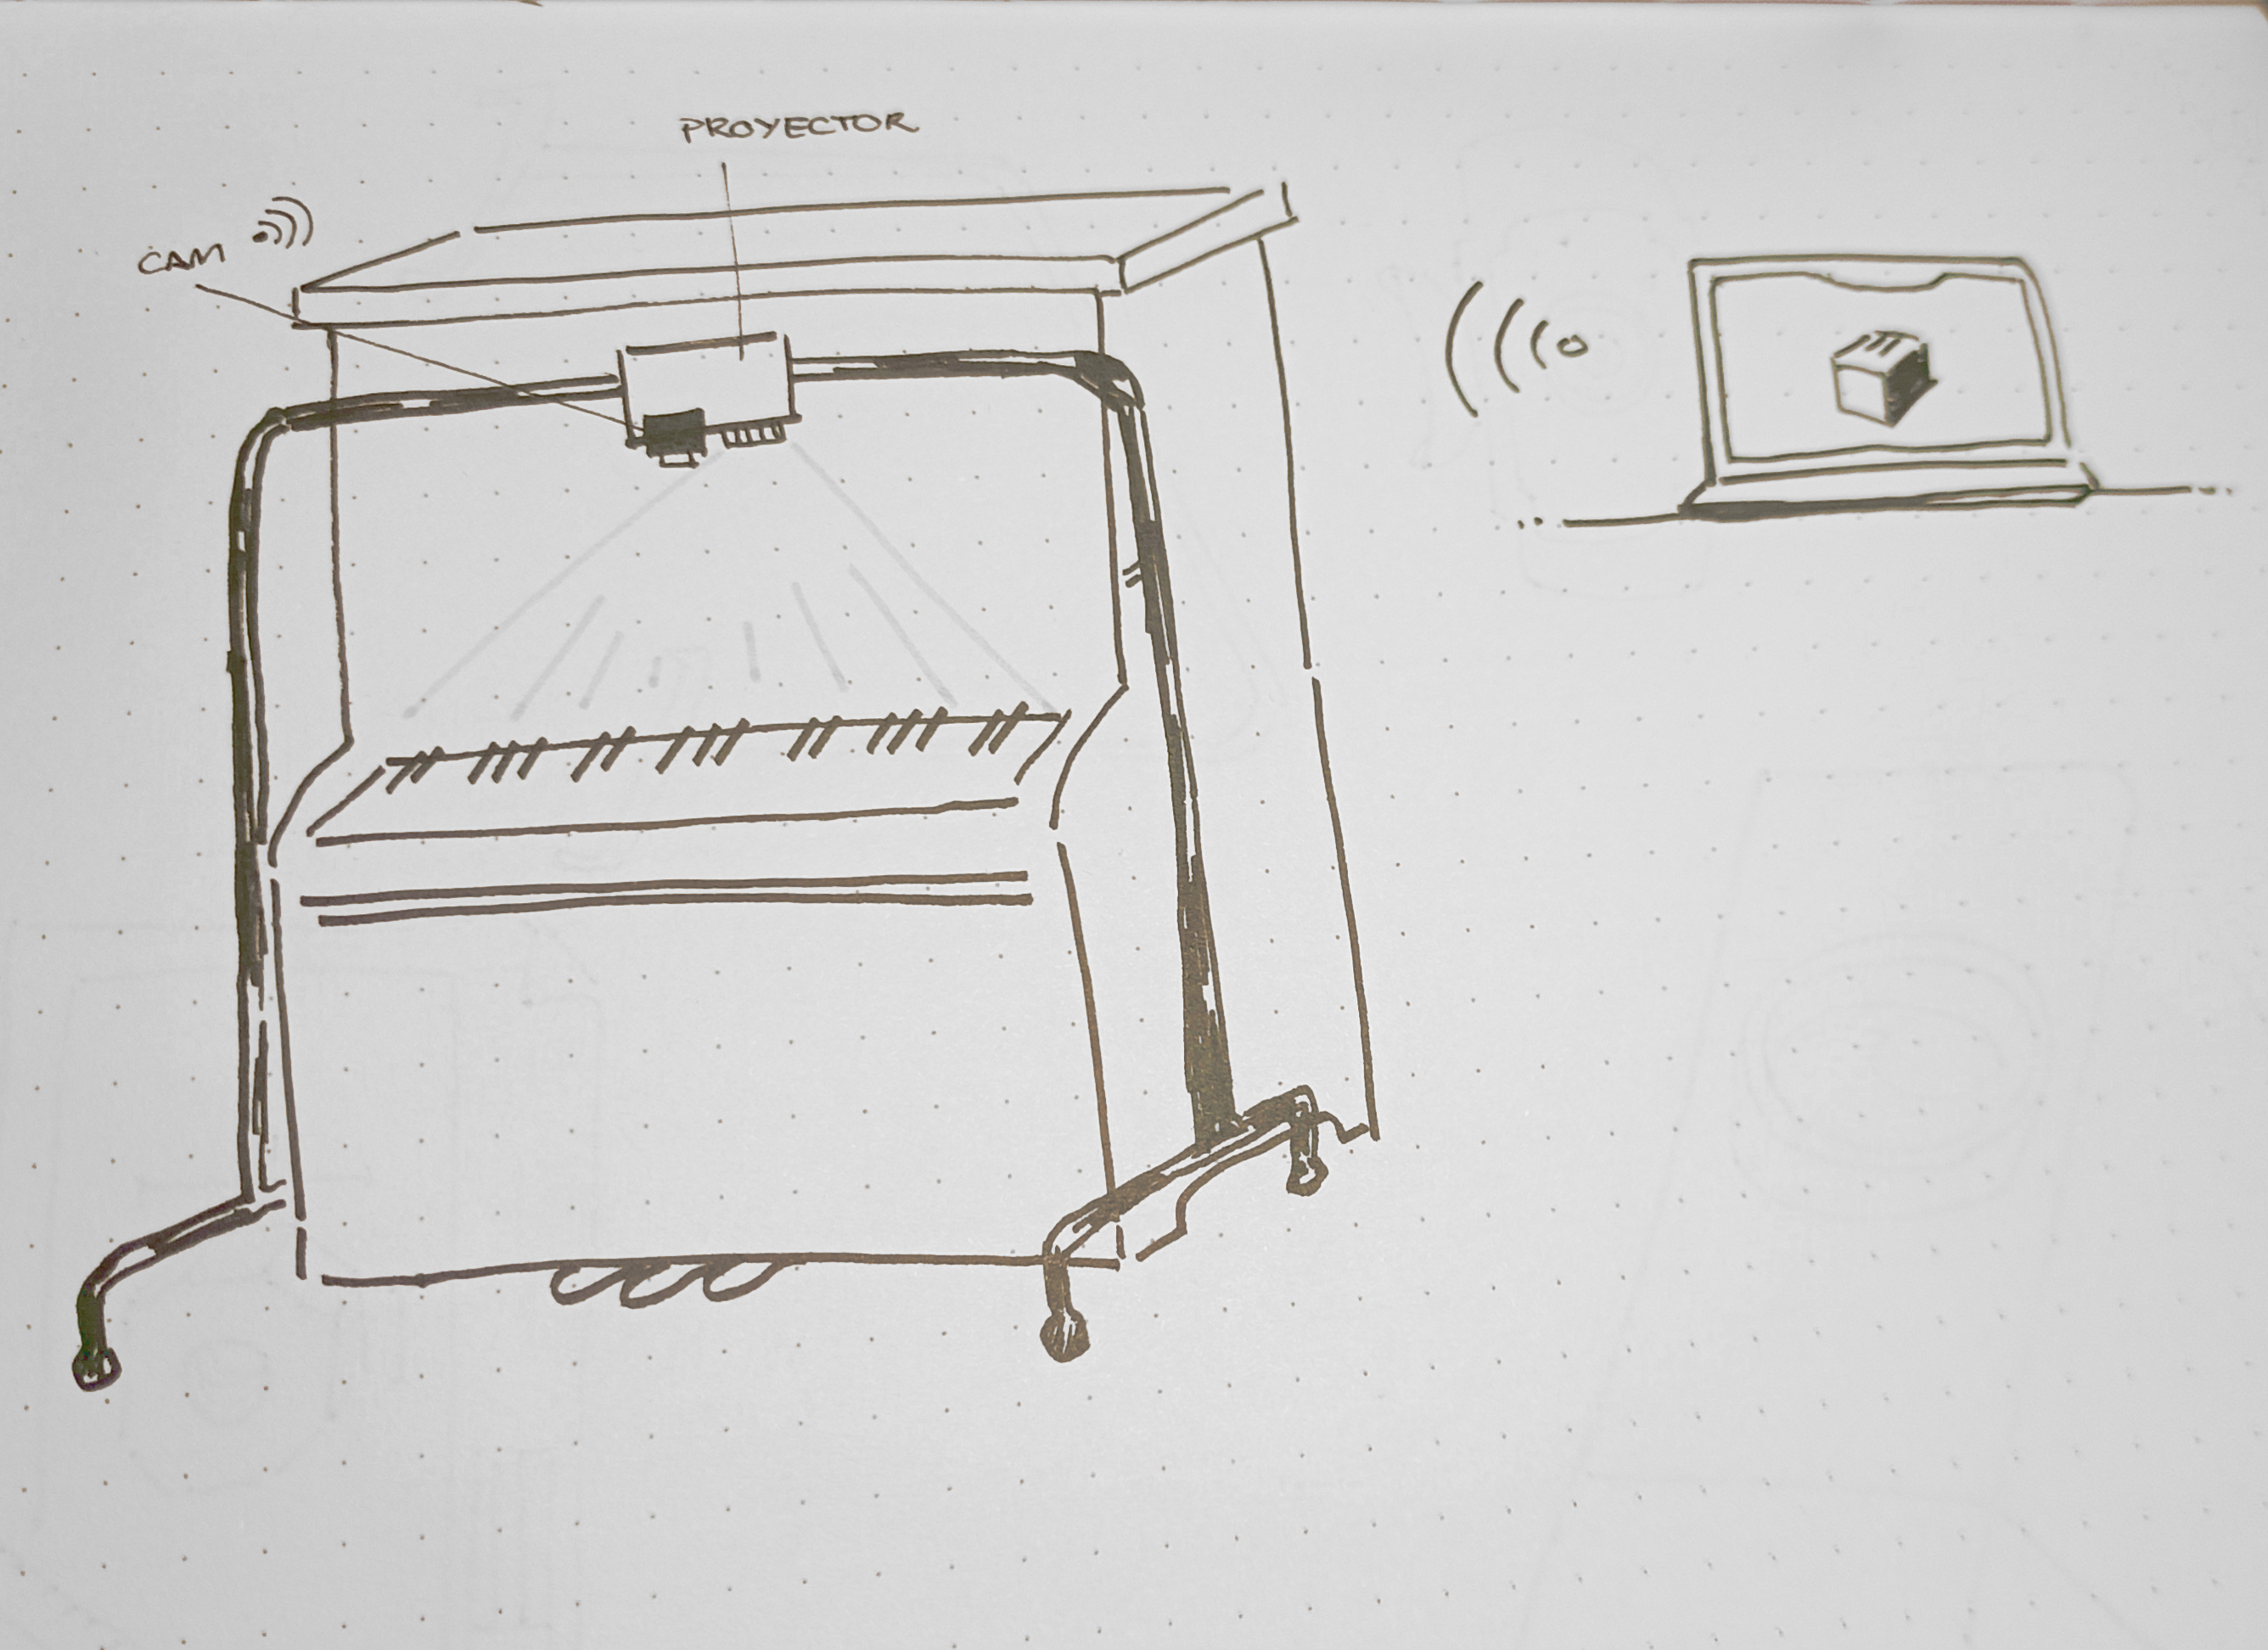
\includegraphics[height=18cm, page=1]{prototipo.png}
    \caption{Prototipo de la versión final}
\end{figure}
